\documentclass[12pt,letterpaper]{exam}
\usepackage[lmargin=1in,rmargin=1in,tmargin=1in,bmargin=1in]{geometry}
\usepackage{../style/exams}

% -------------------
% Course & Exam Information
% -------------------
\newcommand{\course}{MAT 104: Exam 1}
\newcommand{\term}{Spring --- 2024}
\newcommand{\examdate}{02/22/2024}
\newcommand{\timelimit}{85 Minutes}

\setbool{hideans}{false} % Student: True; Instructor: False


% -------------------
% Content
% -------------------
\begin{document}

\examtitle
\instructions{Write your name on the appropriate line on the exam cover sheet. This exam contains \numpages\ pages (including this cover page) and \numquestions\ questions. Check that you have every page of the exam. Answer the questions in the spaces provided on the question sheets. Be sure to answer every part of each question and show all your work. If you run out of room for an answer, continue on the back of the page --- being sure to indicate the problem number.} 
\scores
\bottomline
\newpage


% -------------------
% Questions
% -------------------
\begin{questions}

% Question 1
\newpage
\question[10] Showing all your work and simplifying as much as possible, compute the exact values of the following:
	\begin{enumerate}[(a)]
	\item $6 \div 2(1 + 2)$ \par\vspace{0.3cm}
	\item $\dfrac{-3 - 5(-1)^2 + 12}{-6 - (-8)}$ \par\vspace{0.3cm}
	\item  $(1 - 3)^3 \cdot 4 (7 - 2 \cdot 3)$
	\end{enumerate} \pspace

\sol 
\begin{enumerate}[(a)]
\item 
	\[
	6 \div 2(1 + 2)= 6 \div 2(3)= 3(3)= 9
	\] \pvspace{1.3cm}

\item 
	\[
	\dfrac{-3 - 5(-1)^2 + 12}{-6 - (-8)}= \dfrac{-3 - 5(1) + 12}{-6 + 8}= \dfrac{-3 - 5 + 12}{-6 + 8}= \dfrac{-8 + 12}{-6 + 8}= \dfrac{4}{2}= 2
	\] \pvspace{1.3cm}

\item  
	\[
	\hspace{-1.5cm} (1 - 3)^3 \cdot 4 (7 - 2 \cdot 3)= (-2)^3 \cdot 4 (7 - 2 \cdot 3)= (-2)^3 \cdot 4(7 - 6)= (-2)^3 \cdot 4 (1)= -8 \cdot 4(1)= -32 \cdot 1= -32
	\]
\end{enumerate} 



% Question 2
\newpage
\question[10] Consider the points $A(-7, 6)$, $B(4, -8)$, and $C(5, 1)$. 

\begin{enumerate}[(a)]
\item Plot the points on the graph below, be sure to label each point. 
\item Fill in the missing entries to the non-greyed portion of the chart below. 
\end{enumerate}
	\[
	\fbox{
	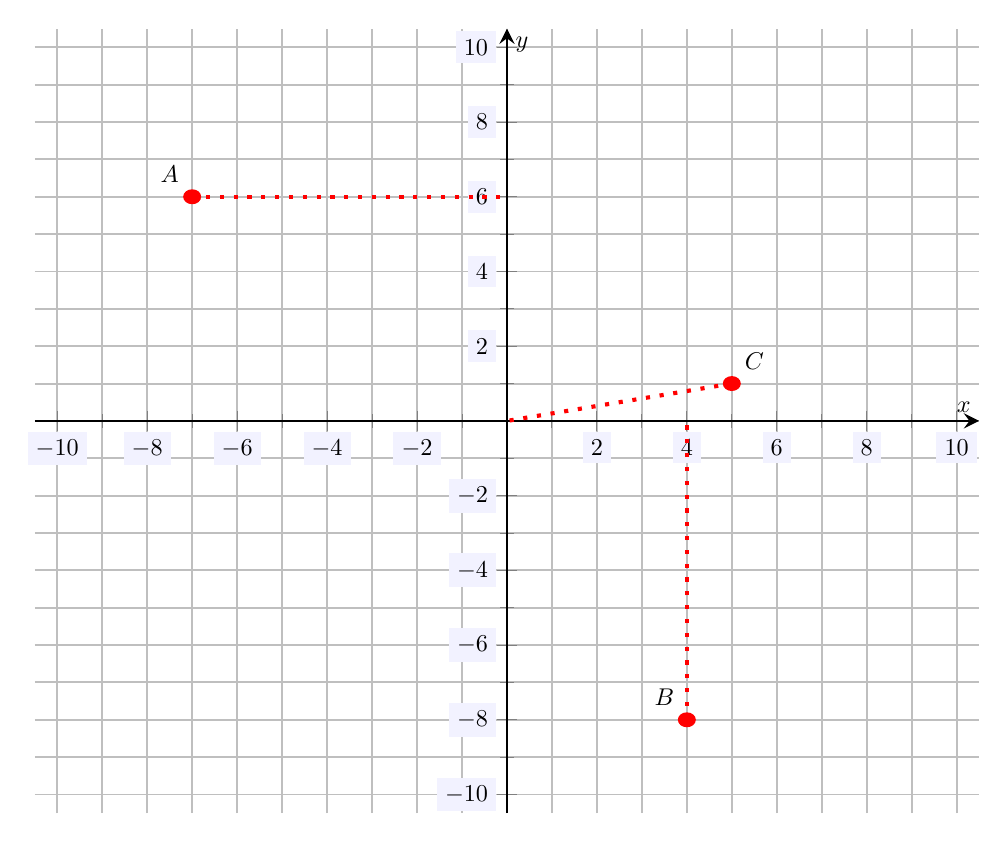
\begin{tikzpicture}[scale=1.75,every node/.style={scale=0.5}]
	\begin{axis}[
	grid=both,
	axis lines=middle,
	ticklabel style={fill=blue!5!white},
	xmin= -10.5, xmax=10.5,
	ymin= -10.5, ymax=10.5,
	xtick={-10,-8,-6,-4,-2,0,2,4,6,8,10},
	ytick={-10,-8,-6,-4,-2,0,2,4,6,8,10},
	minor tick = {-10,-9,...,10},
	xlabel=\(x\),ylabel=\(y\),
	]
	
	\draw[draw=none,fill=red] (-7,6) circle (0.2); \node at (-7.5,6.6) {$A$}; % A
	\draw[draw=none,fill=red] (4,-8) circle (0.2); \node at (3.5,-7.4) {$B$}; % B
	\draw[draw=none,fill=red] (5,1) circle (0.2); \node at (5.5,1.6) {$C$}; % C
	
	\draw[line width=0.03cm,dotted,red] (-7,6) -- (0,6); % A segment
	\draw[line width=0.03cm,dotted,red] (4,-8) -- (4,0); % B segment
	\draw[line width=0.03cm,dotted,red] (5,1) -- (0,0); % C segment
	\end{axis}
	\end{tikzpicture}
	}
	\] 

\begingroup
\renewcommand*{\arraystretch}{2}
\begin{table}[ht]
\begin{tabular}{| >{\centering\arraybackslash}m{1.5cm} | >{\centering\arraybackslash}m{2.5cm} | >{\centering\arraybackslash}m{3.5cm} | >{\centering\arraybackslash}m{3.5cm} | >{\centering\arraybackslash}m{3.5cm} |}
\hline
 & Quadrant & Distance to $x$-axis & Distance to $y$-axis & Distance to origin \\ \hline
Point $A$ & QII & \cellcolor[HTML]{9B9B9B} & $7$ & \cellcolor[HTML]{9B9B9B} \\ \hline
Point $B$ & QIV & $8$ & \cellcolor[HTML]{9B9B9B} & \cellcolor[HTML]{9B9B9B} \\ \hline
Point $C$ & QI & \cellcolor[HTML]{9B9B9B} & \cellcolor[HTML]{9B9B9B} & $\sqrt{26} \approx 5.09902$ \\ \hline
\end{tabular}
\end{table}
\endgroup \pspace

{\itshape\small Recall that the quadrants are labeled counterclockwise starting with I in the upper-right. The distance from a point to a line is the `straight line' distance, i.e. the length of a line segment starting at the point and ending at the line and is perpendicular to the line. Sketching these segments for $A$ and $B$, we can easily find the distance (which must be nonnegative) to the $y$ and $x$-axis, respectively. The distance between two points is the length of the line segment connecting them. To find the distance between points $(x, y)$ and $(a, b)$, we either use $d= \sqrt{(x - a)^2 + (y - b)^2}$ or construct a right triangle using the point to find the distance between them (the segment being the hypotenuse). Using this approach for the point $C$ and the origin, we see we have a right triangle with legs $5$ and $1$. But then the distance to the origin is $\sqrt{5^2 + 1^2}= \sqrt{25 + 1}= \sqrt{26} \approx 5.09902$.}
	
	

% Question 3
\newpage
\question[10] Consider the quadratic function $f(x)= x^2 - 3x + 4$ and the linear function $\ell(x)= 7 - 2x$. Let $\mathcal{I}$ be the interval $\mathcal{I}= [-1, 3]$.
	\begin{enumerate}[(a)]
	\item Find the average rate of change for $f(x)$ on $\mathcal{I}$.
	\item What is the slope of the secant line to $f(x)$ using the points on the graph of $f(x)$ where $x= -1$ and $x= 3$?
	\item Without explicitly calculating the average rate of change, what is the average rate of change for $\ell(x)$ on $\mathcal{I}$?
	\end{enumerate} \pspace

\sol 
\begin{enumerate}[(a)]
\item We know that the average rate of change for a function on an interval is\dots
	\[
	\text{Avg. R.O.C. } f_{[a,b]}= \dfrac{f(b) - f(a)}{b - a}
	\]
We have\dots
	\[
	\begin{aligned}
	f(3)&= 3^2 - 3(3) + 4= 9 - 3(3) + 4= 9 - 9 + 4= 0 + 4= 4 \\
	f(-1)&= (-1)^2 - 3(-1) + 4= 1 - 3(-1) + 4= 1 + 3 + 4= 4 + 4= 8 
	\end{aligned}
	\]
Therefore, we have\dots
	\[
	\text{Avg. R.O.C. } f_{[-1,3]}= \dfrac{f(3) - f(-1)}{3 - (-1)}= \dfrac{4 - 8}{3 + 1}= \dfrac{-4}{4}= -1
	\] \pspace

\item The average rate of change for a function $f(x)$ on $[a, b]$ is the slope of the secant line through the points $\big(a, f(a) \big)$ and $\big(b, f(b) \big)$. From (a), we know that the average rate of change for $f(x)$ on $[-1, 3]$ is $-1$. Therefore, the slope of this secant line is $-1$. \pspace

\item The average rate of change for a function $f(x)$ on $[a, b]$ is the slope of the secant line through the points $\big(a, f(a) \big)$ and $\big(b, f(b) \big)$. However, any two points on a line uniquely determine that line. But then the average rate of change for a linear function over any interval must be constant and equal to its slope. The line $\ell(x)= 7 - 2x$ has slope $m= -2$. Therefore, the average rate of change for $\ell(x)$ on $[-1, 3]$ must be $-2$. We can even verify this:
	\[
	\begin{aligned}
	\ell(3)&= 7 - 2(3)= 7 - 6= 1 \\
	\ell(-1)&= 7 - 2(-1)= 7 + 2= 9 
	\end{aligned}
	\]
	\[
	\text{Avg. R.O.C. } \ell_{[-1,3]}= \dfrac{\ell(3) - \ell(-1)}{3 - (-1)}= \dfrac{1 - 9}{3 + 1}= \dfrac{-8}{4}= -2
	\]
\end{enumerate}



% Question 4
\newpage
\question[10] Consider the linear function $\ell(x)= \frac{2}{3}\, x + 4$.
	\begin{enumerate}[(a)]
	\item Find the slope of $\ell(x)$.
	\item Find the $y$-intercept of $\ell(x)$.
	\item Sketch $\ell(x)$ on the graph below as accurately as possible.
	\item Find the $x$-intercept of $\ell(x)$. 
	\end{enumerate} 

\sol 
\begin{enumerate}[(a)]
\item The slope of a linear function $y= mx + b$ is $m$. We know that $\ell(x)$ is linear with $m= \frac{2}{3}$ and $b= 4$. Therefore, the slope of $\ell(x)$ is $m= \frac{2}{3}$. 

\item The slope of a linear function $y= mx + b$ is $b$. We know that $\ell(x)$ is linear with $m= \frac{2}{3}$ and $b= 4$. Therefore, the $y$-intercept of $\ell(x)$ is $b= 4$, i.e. the $y$-intercept is the point $(0, 4)$. 

\item We know that the line passes through the $y$-intercept, i.e. the point $(0, 4)$. Because $m= \frac{\Delta y}{\Delta x}= \frac{2}{3}$, we can see that for every increase in 3 in $x$, we see an increase of 2 in $y$, i.e. ``right 3, up 2.'' Equivalently, because $\frac{2}{3}= \frac{-2}{-3}$, every decrease of 3 in $x$ results in a decrease of $2$ in $y$, i.e. ``left 3, down 2.'' Using these two rules, we can draw several points and connect them to form an `accurate' line. 

\item From the plot in (c), we can see that the $x$-intercept of $f(x)$ is $x= -6$, i.e. the point $(-6, 0)$. Alternatively, the $x$-intercept(s) occur when $\ell(x)= 0$. But then\dots
	\[
	\begin{gathered}
	\ell(x)= 0 \\
	\tfrac{2}{3}\, x + 4= 0 \\
	\tfrac{2}{3}\,x = -4 \\
	x= -4 \cdot \tfrac{3}{2} \\
	x= -6
	\end{gathered}
	\]
\end{enumerate}

	\vfill

	\[
	\fbox{
	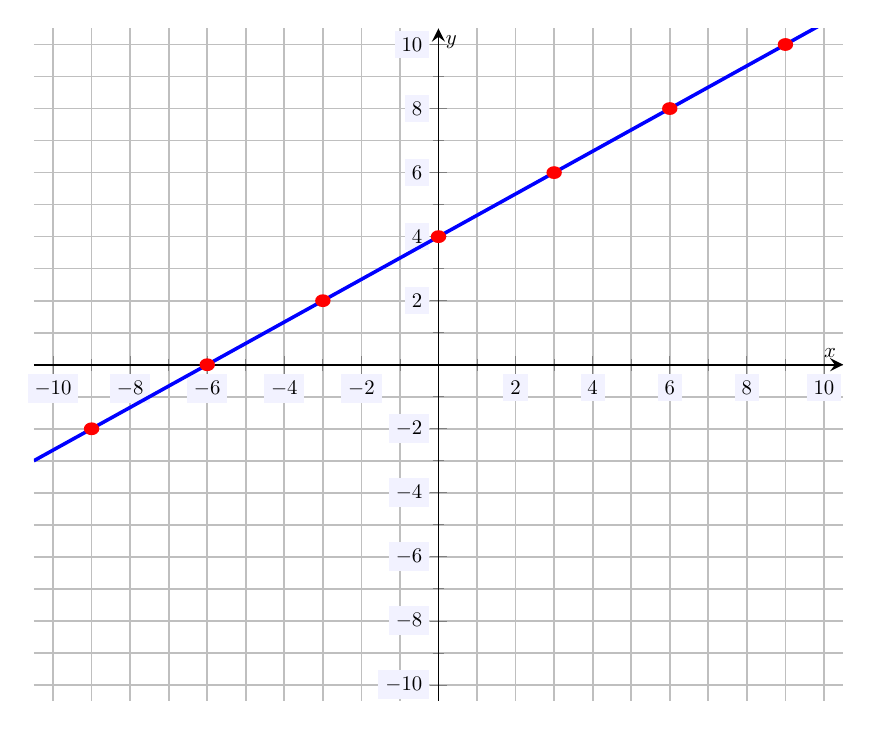
\begin{tikzpicture}[scale=1.5,every node/.style={scale=0.5}]
	\begin{axis}[
	grid=both,
	axis lines=middle,
	ticklabel style={fill=blue!5!white},
	xmin= -10.5, xmax=10.5,
	ymin= -10.5, ymax=10.5,
	xtick={-10,-8,-6,-4,-2,0,2,4,6,8,10},
	ytick={-10,-8,-6,-4,-2,0,2,4,6,8,10},
	minor tick = {-10,-9,...,10},
	xlabel=\(x\),ylabel=\(y\),
	]
	
	\addplot[line width=0.03cm,domain= -10.5:10.5,blue] ({x},{2/3*x + 4});
	
	\draw[draw=none,fill=red] (-9,-2) circle (0.2); 
	\draw[draw=none,fill=red] (-6,0) circle (0.2); 
	\draw[draw=none,fill=red] (-3,2) circle (0.2); 
	\draw[draw=none,fill=red] (0,4) circle (0.2); 
	\draw[draw=none,fill=red] (3,6) circle (0.2); 
	\draw[draw=none,fill=red] (6,8) circle (0.2); 
	\draw[draw=none,fill=red] (9,10) circle (0.2); 
	\end{axis}
	\end{tikzpicture}
	}
	\] 



% Question 5
\newpage
\question[10] Otto Partze owns an automotive parts and repair shop. When a customer brings in a car for service, the amount Otto charges for service is given by $C(t)= 81t + 45$, where $t$ is the number of hours of work done. 
	\begin{enumerate}[(a)]
	\item Find and interpret the slope of $C(t)$. Be sure to include any units.
	\item Find and interpret the $y$-intercept of $C(t)$. Be sure to include any units. 
	\item Find the cost of 90~minutes of service. 
	\end{enumerate} \pspace

\sol 
\begin{enumerate}[(a)]
\item The slope of a linear function $y= mx + b$ is $m$. The function $C(t)= 81t + 45$ is linear with $m= 81$ and $b= 35$. Because $m= \frac{\Delta C}{\Delta t}$, the slope must have units of dollars per hour. Therefore, the slope of $C(t)$ is \$81 per hour. This represents the amount that Otto charges per hour of service, i.e. his hourly rate. \pspace

\item  The $y$-intercept of a linear function $y= mx + b$ is $b$. The function $C(t)= 81t + 45$ is linear with $m= 81$ and $b= 35$. Therefore, the $y$-intercept is 35. Because the $y$-intercept is the value $C(0)$, this has the same units as $C$, i.e. dollars. Therefore, the $y$-intercept is \$35. This is the charge for $t= 0$~hours of service. Therefore, we can interpret this as a `service fee', i.e. a minimal fee to provide any car services. \pspace

\item The function $C(t)$ gives the cost for $t$~\textit{hours} of service. Therefore, we need to express 90~minutes in hours. We know that 90~minutes is $\frac{90}{60}= \frac{3}{2}= 1.5$~hours. We have\dots
	\[
	C(1.5)= 81(1.5) + 45= 121.5 + 45= 166.5
	\]
Therefore, 90~minutes of service would cost \$166.5. 
\end{enumerate}



% Question 6
\newpage
\question[10] Jenna Rossity purchased a new 85" TV for her nephew. The TV cost \$1,599.99. As with any new electronics, the TV depreciates in value by \$372 per year. 
	\begin{enumerate}[(a)]
	\item Find a linear function that gives the resale value of the TV $t$~years from now. 
	\item Find how long until the TV has no resale value. 
	\end{enumerate} \pspace

\sol 
\begin{enumerate}[(a)]
\item The television is currently worth \$1,599.99. Each year, the TV loses \$372 in value. But then after $t$~years, the TV has lost $372t$ dollars in value. But then after $t$~years, the value of the TV in dollars is given by\dots
	\[
	V(t)= 1599.99 - 372t
	\]
We can see that the initial value, \$1,599.99, is the $y$-intercept of the function. The slope of the function represents the amount that the TV's value decreases each year. \pspace

\item The TV has no resale value when it has no value, i.e. when $V(t)= 0$. But then\dots
	\[
	\begin{gathered}
	V(t)= 0 \\[0.3cm]
	1599.99 - 372t= 0 \\[0.3cm]
	372t= 1599.99 \\[0.3cm]
	t \approx 4.30105
	\end{gathered}
	\]
Therefore, the TV will have no resale value after approximately 4.3~years, i.e. 4 years, 3~months, and 18~days. 
\end{enumerate}



% Question 7
\newpage
\question[10] Showing all your work, find the equation of line given in the graph below. If you use any points on the line, be sure that any points you use are \textit{exactly} on the line. 
	\[
	\fbox{
	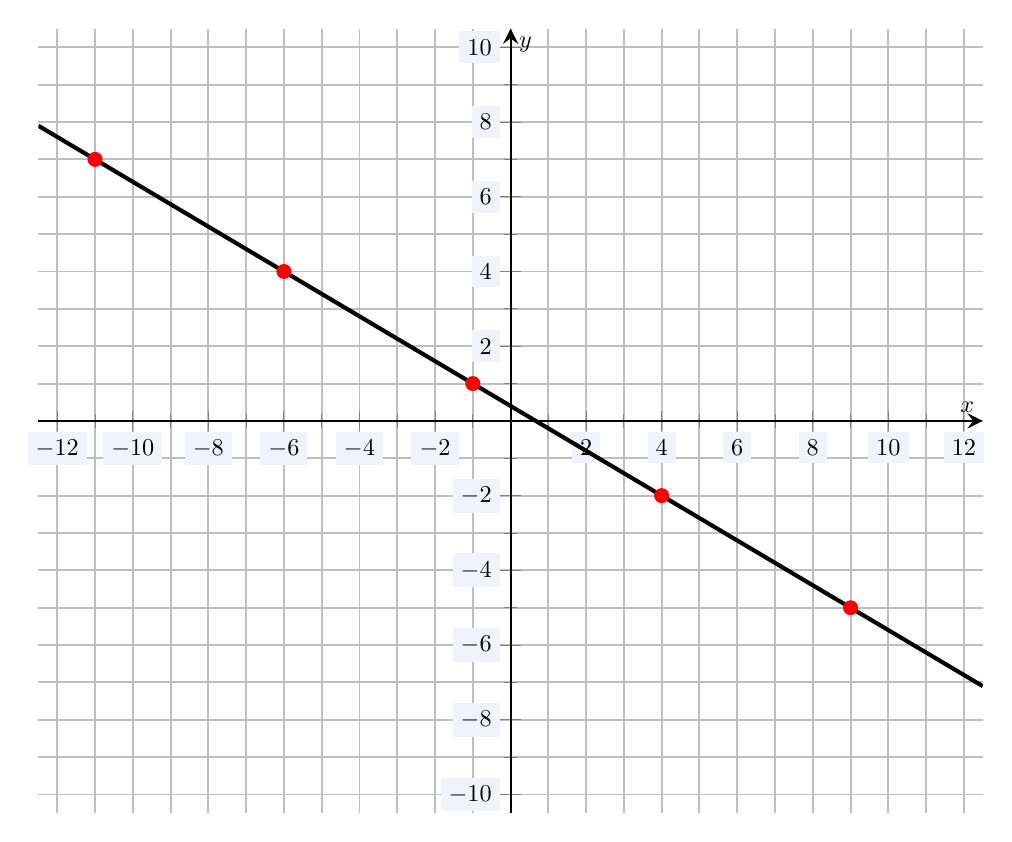
\begin{tikzpicture}[scale=1.75,every node/.style={scale=0.5}]
	\begin{axis}[
	grid=both,
	axis lines=middle,
	ticklabel style={fill=blue!5!white},
	xmin= -12.5, xmax=12.5,
	ymin= -10.5, ymax=10.5,
	xtick={-12,-10,...,12},
	ytick={-12,-10,...,12},
	minor tick = {-12,-11,...,12},
	xlabel=\(x\),ylabel=\(y\),
	]
	\addplot[line width=0.03cm,domain=-12.5:12.5] ({x},{(2 - 3*x)/5});
	
	\draw[draw=none,fill=red] (-11,7) circle (0.2);
	\draw[draw=none,fill=red] (-6,4) circle (0.2);
	\draw[draw=none,fill=red] (-1,1) circle (0.2);
	\draw[draw=none,fill=red] (4,-2) circle (0.2);
	\draw[draw=none,fill=red] (9,-5) circle (0.2);
	\end{axis}
	\end{tikzpicture}
	}
	\] 

\sol Examining the line carefully, we can locate several points \textit{exactly} on the line, marked in red. We shall use the points $(-1, 1)$ and $(4, -2)$. Using these points, we can find the slope of the line:
	\[
	m= \dfrac{\Delta y}{\Delta x}= \dfrac{1 - (-2)}{-1 - 4}= \dfrac{1 + 2}{-1 + (-4)}= \dfrac{3}{-5}= -\dfrac{3}{5}
	\]
But the line contains the point $(x_0, y_0)= (-1, 1)$. Using the point-slope form of the line, we find\dots
	\[
	\begin{aligned}
	y&= y_0 + m(x - x_0) \\[0.3cm]
	&= 1 + \left( -\dfrac{3}{5} \right) \, \big(x - (-1) \big) \\[0.3cm]
	&= 1 - \dfrac{3}{5} \, (x + 1) \\[0.3cm]
	&= 1 - \dfrac{3}{5} \, x - \dfrac{3}{5} \\[0.3cm]
	&= -\dfrac{3}{5} \, x + \dfrac{2}{5} \\[0.3cm]
	&= \dfrac{2 - 3x}{5}
	\end{aligned}
	\]



% Question 8
\newpage
\question[10] Find the exact equation of the line with $x$-intercept $7$ and $y$-intercept $-4$. Express your answer in slope-intercept form. \pspace

\sol Because the $x$-intercept is $7$, the line contains the point $(7, 0)$. Because the $y$-intercept is $-4$, the line contains the point $(0, -4)$. But then the slope is\dots
	\[
	m= \dfrac{\Delta y}{\Delta x}= \dfrac{-4 - 0}{0 - 7}= \dfrac{-4}{-7}= \dfrac{4}{7}
	\]
But then the slope of the line is $\frac{4}{7}$ and the line has $y$-intercept $-4$. Using the slope-intercept form, $y= mx + b$, the line is then\dots
	\[
	y= \dfrac{4}{7} \, x - 4
	\]



% Question 9
\newpage
\question[10] Find the exact equation of the line parallel to the line $y= 9x - 16$ that contains the point $(-1, 7)$. Express your answer in point-slope form. \pspace

\sol The line $y= 9x - 16$ has slope $9$. Because the desired line is parallel to this line, they must have equal slope. But then the slope of the desired line is $m= 9$. We have a line with slope $9$ that contains the point $(-1, 7)$. Using the point-slope form, we have\dots
	\[
	y= y_0 + m(x - x_0)= 7 + 9 \big(x - (-1) \big)
	\]



% Question 10
\newpage
\question[10] Find the exact equation of the line perpendicular to $y= \dfrac{1 - 4x}{2}$ that passes through the $x$-intercept of $f(x)= 4(1 - 3x)$. \pspace

\sol The line $y= \dfrac{1 - 4x}{2}= \dfrac{1}{2} - \dfrac{4x}{2}= \dfrac{1}{2} - 2x$ has slope $-2$. Because the desired line is perpendicular to the line $y= \frac{1 - 4x}{2}$, the slope of the desired line must be the negative reciprocal of the slope of the line $y= \frac{1 - 4x}{2}$. Therefore, the slope of the line must be $m= -\frac{1}{-2}= \frac{1}{2}$. An $x$-intercept of a function $f(x)$ is a point such that $f(x)= 0$. But then\dots
	\[
	\begin{gathered}
	f(x)= 0 \\
	4(1 - 3x)= 0 \\
	1 - 3x= 0 \\
	3x= 1 \\
	x= \dfrac{1}{3}
	\end{gathered}
	\]
Therefore, the line contains the point $(\frac{1}{3}, 0)$. The desired line then has slope $\frac{1}{2}$ and contains the point $(\frac{1}{3}, 0)$. Using the point-slope form, we have\dots
	\[
	y= y_0 + m(x - x_0)= 0 + \dfrac{1}{2} \left(x - \dfrac{1}{3} \right)= \dfrac{1}{2} \, x - \dfrac{1}{6}= \dfrac{3x - 1}{6}
	\]


\end{questions}
\end{document}